% ================================================================
% arXiv preprint
% Selective Hallucination Fragility in Frontier Language Models
% ================================================================
\documentclass[11pt,a4paper]{article}
\usepackage[acceptedWithA]{tacl2021v1}
\usepackage{graphicx}
\graphicspath{{figures/}}
\usepackage{booktabs}
\usepackage{amsmath}
\usepackage{microtype}
\usepackage{xcolor}
\usepackage{caption}
\usepackage{subcaption}       % for side-by-side figures
\captionsetup{font=small,labelfont=bf}

\title{Selective Hallucination Fragility\\ in Frontier Language Models}

\author{Parsa Bakhtary \\
  \texttt{pbakhtary@gmail.com}}

\begin{document}
\maketitle

% ================================================================
% ================================================================
\begin{abstract}
Is hallucination resistance in language models a single capability, or does it fragment into distinct failure modes that can even trade off against each other?
Frontier language models maintain near-perfect numeric fidelity across 20-turn conversations, yet exhibit dramatic, selective failures on other dimensions of context fidelity.
A model achieving 0.995 numeric probe accuracy drops to 0.673 constraint satisfaction after integrating a single revision.
The model with the lowest numeric fidelity (0.890 when re-answering questions it previously computed) achieves the highest source fidelity with zero fabrication and 97.5\% gap abstention (correctly declining to answer when evidence is absent).
When models do fabricate, it is not random. Across 13 missing-evidence gaps, fabrication occurs at 7.7\%, more than double any other gap type.
These findings are paradoxical only if hallucination resistance is a single capability.
Through a three-paradigm framework testing numeric fidelity, constraint satisfaction, and source fidelity across five frontier models in 550 multi-turn conversations, we identify two behaviorally dissociable failure modes that persist despite robust context memory: \emph{constraint maintenance failure}, where models detect conflicts perfectly but cannot integrate revisions; and \emph{epistemic miscalibration}, where fabrication is triggered selectively by implied-evidence gaps.
Cross-paradigm rank concordance is near-zero (Kendall's $W = 0.089$, $p = 0.900$), and the strongest pairwise signal is a significant \emph{inverse} correlation between numeric fidelity and source fidelity ($\rho = -0.895$, $p = 0.040$), suggesting these capabilities may trade off rather than merely vary independently.
\end{abstract}

% ================================================================
\section{Introduction}
\label{sec:intro}
% ================================================================

A natural hypothesis about hallucination in language models is that it reflects a general degradation of context fidelity. As conversations grow longer, models progressively lose track of prior information, and errors of all kinds increase together. Under this hypothesis, a model that excels at one dimension of context fidelity should excel at others. This paper shows that hypothesis is wrong.

We test three dimensions of context fidelity in multi-turn conversation: \emph{numeric fidelity} (can the model correctly re-answer questions whose answers it previously computed?), \emph{constraint satisfaction} (can the model maintain and revise a growing set of constraints?), and \emph{source fidelity} (does the model abstain when evidence is absent, or fabricate?). We present three empirical observations, each of which is paradoxical under the monolithic-degradation view:

\begin{enumerate}
\item \textbf{Selective fragility.} Claude Sonnet~4.5 achieves 0.995 probe accuracy on numeric fidelity across 50 twenty-turn financial analysis conversations, yet in constraint satisfaction tasks, its performance drops from 0.944 to 0.673 after a single constraint revision. We observe a 29-percentage-point collapse on what is structurally a similar task, namely updating prior work in light of new information.

\item \textbf{The capability inversion.} MiniMax~M2.5 ranks last among five frontier models on numeric probe accuracy (0.890 vs.\ 0.995 for the leaders), yet ranks first on source fidelity: zero fabrication, the highest gap abstention (97.5\%), and perfect contradiction resolution. Being worse at tracking numbers predicts being \emph{better} at epistemic judgment.

\item \textbf{Targeted fabrication.} When documents imply that evidence exists without providing it, models fabricate at 7.7\% across 13 such gaps and 65 model-scenario pairs. When documents contain other types of gaps, such as missing numbers, missing reasons, or unstated implications, the same models fabricate at 0--3\%. Fabrication is not a general tendency but a response to a specific gap structure.
\end{enumerate}

A fourth observation sharpens the dissociation:

\begin{enumerate}
\setcounter{enumi}{3}
\item \textbf{The Gemini~2.5~Pro paradox.} Gemini~2.5~Pro achieves the highest per-phase accuracy on numeric computation, yet suffers the steepest post-conflict collapse in constraint satisfaction, dropping from 0.979 to 0.556 after a constraint revision. The same model that best maintains numeric context is the worst at integrating constraint revisions.
\end{enumerate}

These observations are problematic if hallucination resistance degrades uniformly. We resolve them by demonstrating that hallucination comprises at least two behaviorally dissociable failure modes that persist \emph{despite robust context memory}.

\textbf{Constraint maintenance failure:} Models detect conflicts with near-perfect accuracy (0.963--1.000) but cannot integrate revisions into a coherent constraint set. This is not a memory problem, as the model remembers the constraints, but rather an integration problem.

\textbf{Epistemic miscalibration:} Models fabricate in response to a specific gap structure, where ``missing evidence'' implying data exists, rather than randomly. This explains Paradox~2: numeric tracking ability has no bearing on epistemic judgment quality.

The role of numeric fidelity (P1) in our framework is as a \emph{control condition}. P1 demonstrates that models can retrieve their own prior outputs, integrate data revisions, and recompute derived values across 20 turns of conversation. These capacities are prerequisites for constraint integration and epistemic judgment as well. By establishing that they are intact, we narrow the explanatory space. The P2 and P3 failures arise from what is structurally different about those tasks, not from a general degradation of context access.

We establish this through a three-paradigm framework evaluating GPT-4o, Claude Sonnet~4.5, DeepSeek-R1, Gemini~2.5~Pro, and MiniMax~M2.5 across 550 multi-turn conversations containing over 9{,}000 individually scored turns and 100 LLM-judged synthesis evaluations. We release the full experimental framework to support replication.\footnote{Code and data: \url{https://github.com/ilpenzo/hallucination-fragility}}

% ================================================================
\section{Related Work}
\label{sec:related}
% ================================================================

\paragraph{Hallucination taxonomy and evaluation.}
Hallucination in language models has been studied extensively, with comprehensive surveys charting the landscape of intrinsic and extrinsic hallucination across NLG tasks \citep{ji2023survey}. Single-turn benchmarks have been foundational: TruthfulQA \citep{lin2022truthfulqa} targets imitative falsehoods, HaluEval \citep{li2023halueval} covers summarization, dialogue, and question answering, and FActScore \citep{min2023factscore} decomposes long-form generations into atomic claims verified against knowledge sources. Large-scale evaluation suites such as HELM \citep{liang2023helm} and BIG-Bench \citep{srivastava2023beyond} assess broad capabilities but typically within single-turn interactions. These benchmarks evaluate isolated queries, whereas our framework tests sustained multi-turn interactions where earlier outputs become inputs to later reasoning.

\paragraph{Long-context faithfulness.}
\citet{liu2024lost} demonstrated that language models struggle to use information positioned in the middle of long contexts, establishing position-dependent retrieval as a fundamental limitation. Our work extends this from static document retrieval to dynamic multi-turn conversation, where the information to be maintained includes the model's own prior outputs. The distinction matters, as multi-turn fidelity requires the model to treat its own prior outputs as inputs to subsequent reasoning, not merely retrieve information provided by the user.

\paragraph{Multi-turn and planning evaluation.}
MT-Bench \citep{zheng2023judging} tests conversational quality but not factual consistency across turns. DiaHalu \citep{chen2024diahalu} evaluates dialogue-level hallucination, and recent graph-based methods detect contextual inconsistencies in conversation \citep{rathore2026temporal}. In the planning domain, benchmarks such as TravelPlanner \citep{xie2024travelplanner} and PlanBench \citep{valmeekam2023planbench} evaluate multi-constraint satisfaction, though typically in single-turn settings. Our P2 paradigm extends this to multi-turn constraint accumulation with mid-conversation conflict, testing whether models can \emph{revise} a constraint set rather than merely satisfy a static one.

\paragraph{LLM-as-judge methodology.}
Using LLMs as evaluators has become standard following G-Eval \citep{liu2023geval} and the Chatbot Arena framework \citep{chiang2024chatbot}. We employ an LLM judge for our synthesis paradigm with cross-provider validation (\S\ref{sec:p3}). Our cross-paradigm concordance uses Kendall's~$W$ \citep{kendall1939problem}.

% ================================================================
\section{Experimental Design}
\label{sec:design}
% ================================================================

We constructed three experimental paradigms, each isolating a distinct dimension of \emph{context fidelity}, the ability to maintain accurate representations of information within a conversation. All paradigms use 20-turn conversations conducted programmatically via each model's API. Scenario construction prioritized experimental control over naturalistic appearance. P1 scenarios were generated programmatically, using a template-based generator produces synthetic company financial data with 15 question types and pre-computed ground truth, enabling automatic scoring. P2 scenarios use a reverse-generation architecture: a feasible solution is generated first and constraints are derived from it, guaranteeing satisfiability without requiring a constraint solver. P3 document sets were constructed manually with planted contradictions and annotated information gaps. All scenarios are synthetic, and we address the generalization implications in \S\ref{sec:conclusion}.

\subsection{Paradigm~1: Progressive Numerical Analysis}
\label{sec:p1}

Each of 50 scenarios presents a fictional company's quarterly financial data and poses 20 questions of increasing complexity across four phases. There are direct lookups (turns 1--4, hereafter T1--T4), single-step derivations such as margins and ratios (T5--T10), multi-step computations including cumulative sums and top-$k$ rankings (T11--T18), and a correction phase where the user provides an updated data value and asks the model to recompute a prior answer (T19--T20).

Probe questions at turns 5, 10, 15, and 20 re-ask questions whose answers the model computed earlier, testing self-output retrieval. Accuracy is scored against precomputed ground truth with a 1\% tolerance. We validated this threshold by computing mean absolute percentage error (MAPE) across all 2{,}879 scored numeric turns: the error distribution is bimodal, with 98.4\% of turns showing $<$1\% error and only 0.1\% showing $>$50\% error. Median APE is 0.0\% for all five models; MAPE ranges from 0.002\% (Claude Sonnet~4.5) to 0.43\% (MiniMax~M2.5). The binary metric captures the relevant variation because errors are either near-zero or catastrophic.

\subsection{Paradigm~2: Constraint Satisfaction Under Load}
\label{sec:p2}

Each of 40 scenarios presents a scheduling task with constraints that accumulate over 20 turns. At checkpoint turns 6, 11, 17, and 20, the model produces a complete plan, automatically verified against all active constraints. Between turns 11 and 17, a conflict is introduced: a new constraint contradicts an earlier one, and the model is told which to override. This tests selective updating of internal representations.

Plans were parsed using a format-tolerant extractor handling markdown, bullet lists, natural language formatting, and chain-of-thought traces. Parser choice affects absolute satisfaction levels (a stricter parser reduces scores by approximately 15--20 points for the most format-variable models) but preserves relative rankings with one minor exception. This design reflects a key methodological principle, namely that evaluation should measure constraint satisfaction, not format adherence.

\subsection{Paradigm~3: Multi-Document Synthesis}
\label{sec:p3}

Each of 20 scenarios provides 3--5 documents on a shared topic spanning legal, scientific, technical, and financial domains. Each scenario contains planted contradictions, information gaps (where a plausible question has no answer in the sources), and an authority manipulation where a high-status source either supports or contradicts the evidence. In 7 scenarios the authority is correct, while in 13 it is wrong.

Responses were evaluated by Claude Opus~4.6 as an LLM judge, scoring contradiction identification and resolution, gap abstention (whether the model correctly declines to answer when the sources lack sufficient evidence) versus fabrication (whether it invents unsupported claims), and authority deference (whether the model gives undue weight to high-status sources over contradicting evidence). To validate reliability, all 100 entries were independently re-judged by GPT-5.2 (OpenAI) using the identical rubric. Overall binned agreement was 97.2\% across 400 paired dimension scores, with Gwet's AC1 $= 0.971$. On the two dimensions with sufficient marginal variance for standard $\kappa$, gap abstention ($\kappa_{\mathrm{lin}} = 0.877$) and fabrication ($\kappa = 0.712$), agreement was substantial to almost perfect. Full reliability results are in Appendix~\ref{app:irr}.

\subsection{Models, Parameters, and Scale}
\label{sec:params}

Five frontier models, GPT-4o (\texttt{gpt-4o-2024-11-20}), Claude Sonnet~4.5 (\texttt{claude-sonnet-4-5-20250929}), DeepSeek-R1 (\texttt{deepseek-reasoner}), Gemini~2.5~Pro (\texttt{gemini-2.5-pro}), and MiniMax~M2.5 (\texttt{MiniMax-M2.5}), each completed all 50 P1, 40 P2, and 20 P3 scenarios, yielding 550 conversations with over 9{,}000 scored turns and 100 LLM-judged synthesis evaluations. All models were run at temperature 0.0, standard for factual and reasoning evaluations \citep{lin2022truthfulqa,liang2023helm} where sampling noise is a confound; the targeted replication (\S\ref{sec:conclusion}) partially addresses variance concerns. Maximum output tokens were 2{,}048 (16{,}384 for DeepSeek-R1, 8{,}192 for Gemini~2.5~Pro) to accommodate model-specific verbosity: DeepSeek-R1 produces extended chain-of-thought traces (mean 1{,}135 tokens) and Gemini~2.5~Pro is similarly expansive, yet both operated well within budget (64\% and 17.5\% utilization). Among the 2{,}048-ceiling models, Claude Sonnet~4.5 hit the limit on 17 of 2{,}040 turns (0.8\%, all on T19 where scored content precedes the truncation point), MiniMax~M2.5 on 6 turns (0.3\%, all non-scored), and GPT-4o never reached the ceiling. Each paradigm used a task-appropriate system prompt: a financial analyst persona for P1, a planning assistant for P2, and an expert analyst for P3 (full prompts in supplementary materials). Each model-scenario combination was run once.

% ================================================================
\section{Results}
\label{sec:results}
% ================================================================

We organize results around two behaviorally dissociable failure modes, preceded by the P1 control condition establishing that numeric context fidelity is robust, then present cross-paradigm evidence of their dissociability.

% ----------------------------------------------------------------
\subsection{Numeric Fidelity: The Control Condition}
\label{sec:numeric}

Across 50 scenarios per model, probe accuracy, the rate at which models correctly answer questions whose answers they previously computed, ranges from 0.890 (MiniMax~M2.5) to 0.995 (Claude Sonnet~4.5, DeepSeek-R1). These are not ceiling effects on trivial questions, but rather are probes that re-ask lookups, single-step derivations, multi-step aggregations, and correction propagation problems across conversations of 20 turns.

\begin{table*}[tbp]
\centering
\caption{P1 probe accuracy and phase-level accuracy across question types. All models maintain high accuracy across all phases, establishing that numeric context fidelity is robust over 20-turn conversations.}
\label{tab:p1-accuracy}
\small
\begin{tabular}{lccccc}
\toprule
\textbf{Model} & \textbf{Probe} & \textbf{Lookup} & \textbf{Single} & \textbf{Multi} & \textbf{Corr.} \\
 & \textbf{Acc.} & (T1--5) & (T5--10) & (T11--15) & (T19--20) \\
\midrule
Sonnet 4.5      & \textbf{0.995} & 0.962 & 1.000 & 0.971 & 0.990 \\
DeepSeek-R1     & \textbf{0.995} & 0.974 & 0.992 & 0.968 & 0.983 \\
Gemini 2.5 Pro  & 0.965          & 0.980 & 1.000 & 0.968 & 0.962 \\
GPT-4o          & 0.955          & 0.908 & 1.000 & 0.899 & 0.880 \\
MiniMax M2.5    & 0.890          & 0.952 & 0.996 & 0.883 & 0.867 \\
\bottomrule
\end{tabular}
\end{table*}

Table~\ref{tab:p1-accuracy} shows uniformly high performance across all question phases. Several patterns merit note. First, single-step derivations (margins, ratios, growth rates) are answered at 0.992--1.000 by all models, indicating that basic financial computation within conversation is essentially solved. Second, correction propagation, where the model must integrate a data revision and recompute a prior answer, remains above 0.867 for all models. Even the weakest model (MiniMax~M2.5) propagates corrections successfully 87\% of the time. Third, the remaining errors (66 out of approximately 4{,}000 scored turns across all models) cluster in specific subtypes: conditional aggregations requiring multiple filtering steps (e.g., ``What is the total revenue across quarters where gross margin exceeded 40\%?'') and count-above queries (e.g., ``How many quarters had operating expenses above \$50M?'') where models occasionally miscount by one.

This establishes the baseline for interpreting the P2 and P3 results. When models fail at constraint maintenance or epistemic judgment, the explanation is not that they have lost access to conversational context. P1 demonstrates that models can retrieve their own prior outputs, integrate data revisions, and recompute derived values across 20 turns. These are the very capacities that constraint integration and epistemic judgment also require. The failures in P2 and P3 must therefore arise from what is structurally different about those tasks, not from what they share with P1.

% ----------------------------------------------------------------
\subsection{Failure Mode~1: Constraint Maintenance}
\label{sec:constraint}

The P2 paradigm measures a qualitatively different challenge: maintaining a growing constraint set after a mid-conversation conflict forces selective revision. The results reveal a sharp dissociation between \emph{detecting} conflicts and \emph{integrating} revisions.

\begin{figure*}[tbp]
\centering
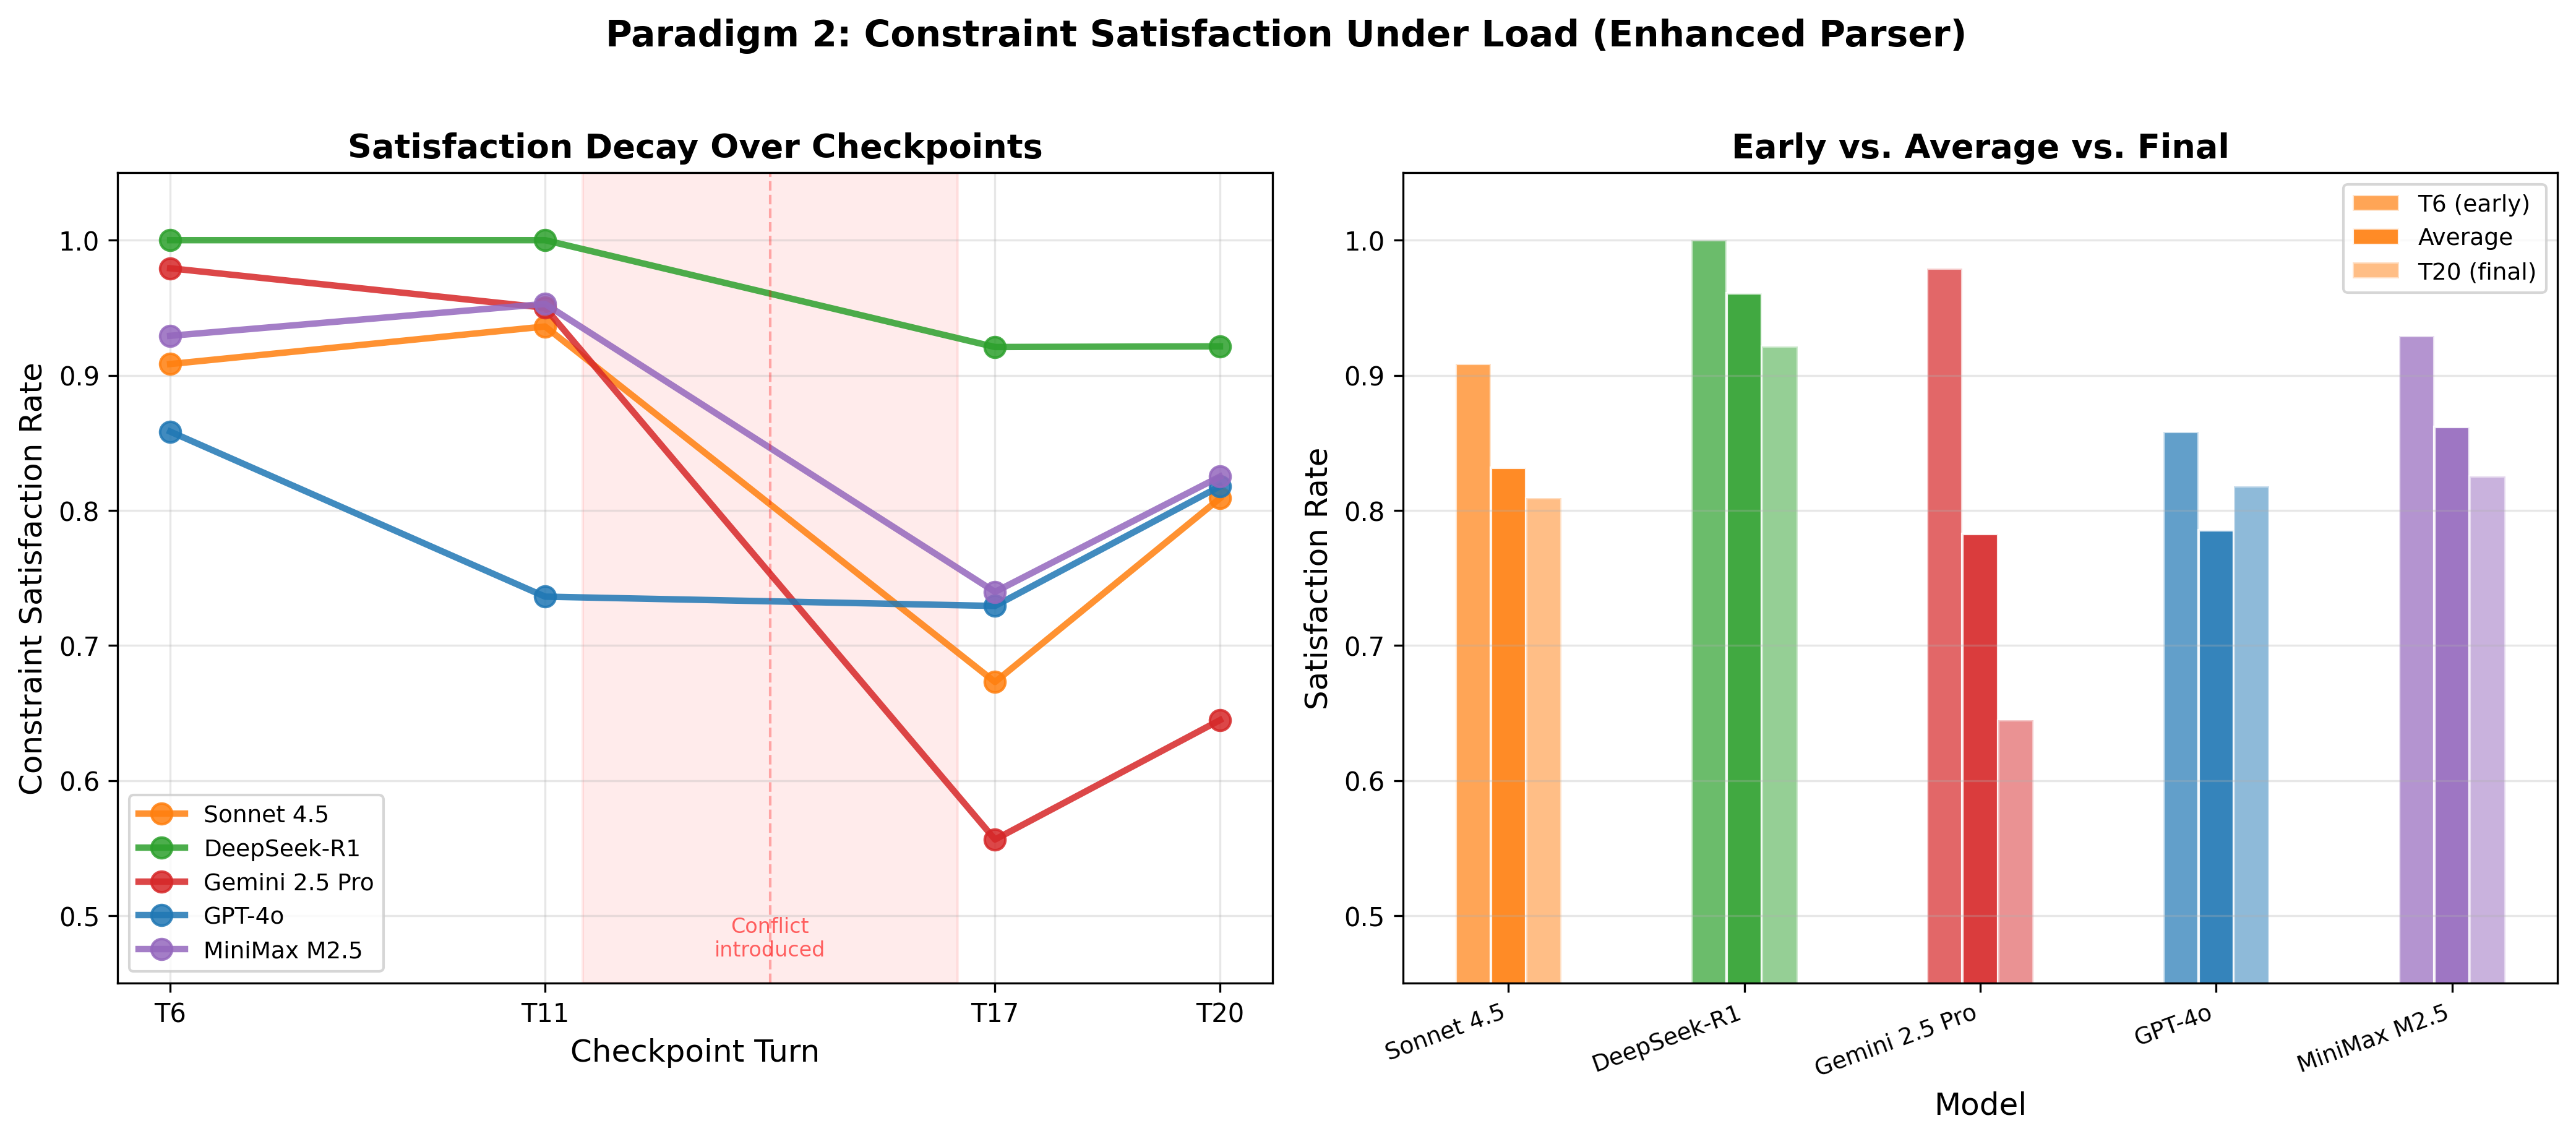
\includegraphics[width=\textwidth]{p2_decay_curves.png}
\caption{P2 satisfaction across checkpoints. Dashed line: conflict introduction. DeepSeek-R1 maintains near-perfect satisfaction. Gemini~2.5~Pro shows the steepest post-conflict collapse despite strong pre-conflict performance.}
\label{fig:p2-decay}
\end{figure*}

\begin{table}[tbp]
\centering
\caption{P2 constraint satisfaction. Conflict detection is uniformly high (0.963--1.000); post-revision satisfaction varies dramatically, revealing that detection and integration are dissociable.}
\label{tab:p2}
\footnotesize
\begin{tabular}{lcccc}
\toprule
\textbf{Model} & \textbf{Avg} & \textbf{Conf.} & \textbf{T17} & \textbf{T20} \\
 & \textbf{Sat.} & \textbf{Det.} & \textbf{Sat.} & \textbf{Sat.} \\
\midrule
DeepSeek-R1     & \textbf{0.961} & 0.969          & 0.921 & 0.921 \\
MiniMax M2.5    & 0.862          & 0.981          & 0.740 & 0.825 \\
Sonnet 4.5      & 0.832          & \textbf{1.000} & 0.673 & 0.809 \\
GPT-4o          & 0.785          & \textbf{1.000} & 0.729 & 0.818 \\
Gemini 2.5 Pro  & 0.782          & 0.963          & 0.556 & 0.645 \\
\bottomrule
\end{tabular}
\end{table}

DeepSeek-R1 dominates with 0.961 average satisfaction, maintaining above 0.92 at every checkpoint. The critical finding is the detection--integration dissociation: conflict detection is uniformly high (0.963--1.000), yet post-conflict satisfaction varies from 0.921 (DeepSeek-R1) to 0.556 (Gemini~2.5~Pro) at T17. All models detect contradictions, and few integrate the revision successfully.

This dissociation parallels P1's correction propagation but with dramatically different outcomes: correction succeeds 87--99\% of the time in P1, while constraint revision succeeds only 56--92\% in P2. The difference is structural, since numeric correction updates a single cached value, while constraint revision requires maintaining all prior constraints while selectively modifying one, and models fail at the latter even when context memory (as demonstrated by P1) is intact.

Gemini~2.5~Pro's performance is particularly informative. It achieves the second-highest initial satisfaction (0.979 at T6) but suffers the steepest post-conflict collapse, never recovering above 0.645. The same model that maintains among the highest numeric fidelity in P1 (0.965 probe accuracy, 1.000 single-step, 0.962 correction) is the \emph{worst} at maintaining constraint revisions in P2. This confirms that numeric fidelity and constraint integration are behaviorally dissociable: they draw on different capabilities, and excellence at one does not predict competence at the other.

A concrete example illustrates the dissociation. On a conference scheduling task (P2\_002), Gemini~2.5~Pro maintains perfect constraint satisfaction through T11, then at T15 responds to a new constraint with ``\textsc{conflict detected}'' and a detailed multi-paragraph analysis of exactly why the constraints are incompatible. Yet at T17, when asked to produce an updated plan, the model refuses, asserting ``It is currently impossible to create a plan" and listing conflicts rather than resolving them by overriding the superseded constraint. Satisfaction drops from 1.000 to 0.083. The model's understanding of the conflict is flawless, yet its ability to act on that understanding is not.

% ----------------------------------------------------------------
\subsection{Failure Mode~2: Epistemic Miscalibration}
\label{sec:epistemic}

The second failure mode is qualitatively different from constraint maintenance. Constraint failure is a problem of \emph{integration}, in that the model remembers the constraints but cannot reconcile them. Epistemic miscalibration is a problem of \emph{judgment}, where they fabricate an answer when the model should acknowledge uncertainty. This distinction resolves the capability inversion, as MiniMax~M2.5's relatively lower numeric fidelity has no bearing on the quality of its epistemic judgment.

\begin{table*}[tbp]
\centering
\caption{P3 multi-document synthesis results. All models achieve zero inappropriate authority deference. MiniMax~M2.5, the weakest numeric tracker, leads on every source fidelity metric.}
\label{tab:p3}
\small
\begin{tabular}{lccccc}
\toprule
\textbf{Model} & \textbf{Contr.\ Res.} & \textbf{Gap Abst.} & \textbf{Fab.\ Rate} & \textbf{Appr.\ Def.} & \textbf{Inappr.\ Def.} \\
\midrule
Sonnet 4.5      & 0.980 & 0.885 & 0.050 & 86\% & 0\% \\
DeepSeek-R1     & 1.000 & 0.875 & 0.100 & 100\% & 0\% \\
Gemini 2.5 Pro  & 1.000 & 0.930 & \textbf{0.000} & 100\% & 0\% \\
GPT-4o          & 0.973 & 0.875 & 0.100 & 86\% & 0\% \\
MiniMax M2.5    & 1.000 & \textbf{0.975} & \textbf{0.000} & 100\% & 0\% \\
\bottomrule
\end{tabular}
\end{table*}

Table~\ref{tab:p3} presents the full P3 results. All five models achieved near-perfect contradiction identification (1.000) and resolution (0.973--1.000). Gap abstention ranged from 0.875 (DeepSeek-R1 and GPT-4o) to 0.975 (MiniMax~M2.5). Fabrication rates were low but non-zero for three models: Claude Sonnet~4.5 at 5\%, DeepSeek-R1 and GPT-4o at 10\%, while Gemini~2.5~Pro and MiniMax~M2.5 produced zero fabrications. On authority bias, across 13 scenarios where the high-authority source was wrong, \emph{every model scored zero inappropriate deference}. No model was misled by status alone. In the 7 scenarios where authority was correct, all models deferred appropriately at 100\%, except Claude Sonnet~4.5 and GPT-4o at approximately 86\%, which is a mild over-skepticism rather than a failure of reasoning.

\paragraph{Implication-to-certainty collapse.}
The key finding is that fabrication is not random but triggered by a specific gap structure. We classified the 20 information gaps across the core P3 scenarios into five types by what information is missing. An initial analysis revealed that all fabrication events concentrated in ``missing evidence'' gaps, where sources imply that supporting evidence exists without providing it. To test this pattern at larger sample size, we constructed 8 additional missing-evidence scenarios (P3\_021--P3\_028, included in the released dataset) spanning scientific, legal, and technical domains and ran all five models on them, expanding the missing-evidence sample from 5 to 13 gaps (65 model-scenario pairs) while leaving the other gap types unchanged.

Across the expanded sample, missing-evidence gaps produce a fabrication rate of 0.077 (5 events in 65 pairs), more than double the next most vulnerable type. ``Missing detail'' gaps ($N = 6$) trigger fabrication at 0.033, while ``missing number'' ($N = 5$), ``missing reason'' ($N = 2$), and ``implied not stated'' ($N = 2$) gaps all yield zero fabrication across a combined 45 model-scenario pairs. We term this \emph{implication-to-certainty collapse}, that is to say when a gap sits at the boundary between what is stated and what is implied, models bridge the gap by converting a qualified implication into a fabricated certainty. When gaps involve missing numbers, reasons, or unstated implications (gap types that lack the implied-evidence structure), the models abstain correctly. Fabrication concentrates further within the missing-evidence type, as show by 5 of the 13 missing-evidence scenarios triggering at least one fabrication event, indicating that not all implied-evidence gaps are equally provocative but that the phenomenon recurs across diverse scenarios and domains.

As a concrete example, one scenario (P3\_019) presented clinical trial documents where an internal memo stated that human trials ``excluded drinkers,'' and a gap probe asked whether any human participants consumed alcohol. Three of five models responded with a definitive ``no'', converting an enrollment exclusion criterion (who was \emph{eligible} to participate) into a behavioral claim about what participants \emph{did} (whether anyone consumed alcohol during the study). The fabrication is subtle, given the model's response is consistent with the documents' implications but states as certainty what the documents only imply.

A second example from the legal domain illustrates the same mechanism in a different setting. In P3\_008, a cease-and-desist letter states ``we have evidence you created [the algorithm] while employed by us'' but never specifies what that evidence is. When asked what evidence the company possessed, DeepSeek-R1 confidently identified ``the founder's own public admission'' from a blog post, fabricating a specific causal link between two documents that no source actually establishes. The correct answer is that the evidence is unknown, since the letter references it but does not describe it. As with P3\_019, the fabrication is plausible and consistent with the documents' implications, but states as fact what the sources only suggest.

Perhaps surprisingly, the domain predicts vulnerability. Scientific scenarios were fabricated at the highest rate, followed by legal and technical, while corporate scenarios produced zero fabrication. This scenario-level clustering, combined with the gap-type specificity across the expanded sample, suggests that fabrication is driven by specific textual features that invite over-inference rather than by general model weakness.

% ----------------------------------------------------------------
\subsection{Cross-Paradigm Dissociability}
\label{sec:cross}

The preceding sections established two behaviorally dissociable failure modes that persist despite robust numeric context fidelity. We now examine whether these capabilities covary across models.

\begin{table}[tbp]
\centering
\caption{Cross-paradigm summary. Rankings shift across paradigms shows no model dominates. The ranks are in parentheses, with ties receiving the average of the tied positions (e.g., two models tied for 1st are each ranked 1.5).}
\label{tab:cross}
\scriptsize
\begin{tabular}{lccr}
\toprule
\textbf{Model} & \textbf{P1 Probe} & \textbf{P2 Sat.} & \textbf{P3 Abst.} \\
\midrule
Sonnet 4.5      & \textbf{.995} (1.5) & .832 (3) & .885 (3) \\
DeepSeek-R1     & \textbf{.995} (1.5) & \textbf{.961} (1) & .875 (4.5) \\
Gemini 2.5 Pro  & .965 (3)   & .782 (5) & .930 (2) \\
GPT-4o          & .955 (4)   & .785 (4) & .875 (4.5) \\
MiniMax M2.5    & .890 (5)   & .862 (2) & \textbf{.975} (1) \\
\bottomrule
\end{tabular}
\end{table}

Kendall's $W$ across five models on three paradigm metrics yields $W = 0.089$ ($\chi^2 = 0.533$, $df = 4$, $p = 0.900$), indicating near-zero concordance: knowing a model's rank on one paradigm provides essentially no information about its rank on another. The pairwise Spearman correlations tell a more specific story. P1--P2 ($\rho = -0.051$, $p = 0.935$) and P2--P3 ($\rho = -0.154$, $p = 0.805$) show no relationship whatsoever. P1--P3 ($\rho = -0.895$, $p = 0.040$), however, reveals a strong and significant \emph{inverse} correlation. Models with the highest numeric fidelity tend to have the lowest source fidelity, and vice versa. This is not a complication for the dissociability thesis but a sharpening of it. Zero correlation would indicate mere independence, but a significant negative correlation suggests these capabilities may trade off, perhaps because the training or architectural properties that support precise numeric tracking are distinct from, or even in tension with, those that support conservative epistemic judgment. The internal P3 metrics show strong consistency ($\rho = 0.973$, $p = 0.005$ between gap abstention and fabrication rate), confirming that P3 measures a coherent capability.

The rank inversions in Table~\ref{tab:cross} are pervasive. MiniMax~M2.5 ranks last on P1 but first on P3, Gemini~2.5~Pro ranks 3rd on P1 but last on P2, and no model's standing on one paradigm predicts its standing on another.

\begin{figure*}[tbp]
\centering
\begin{subfigure}[t]{0.48\textwidth}
  \centering
  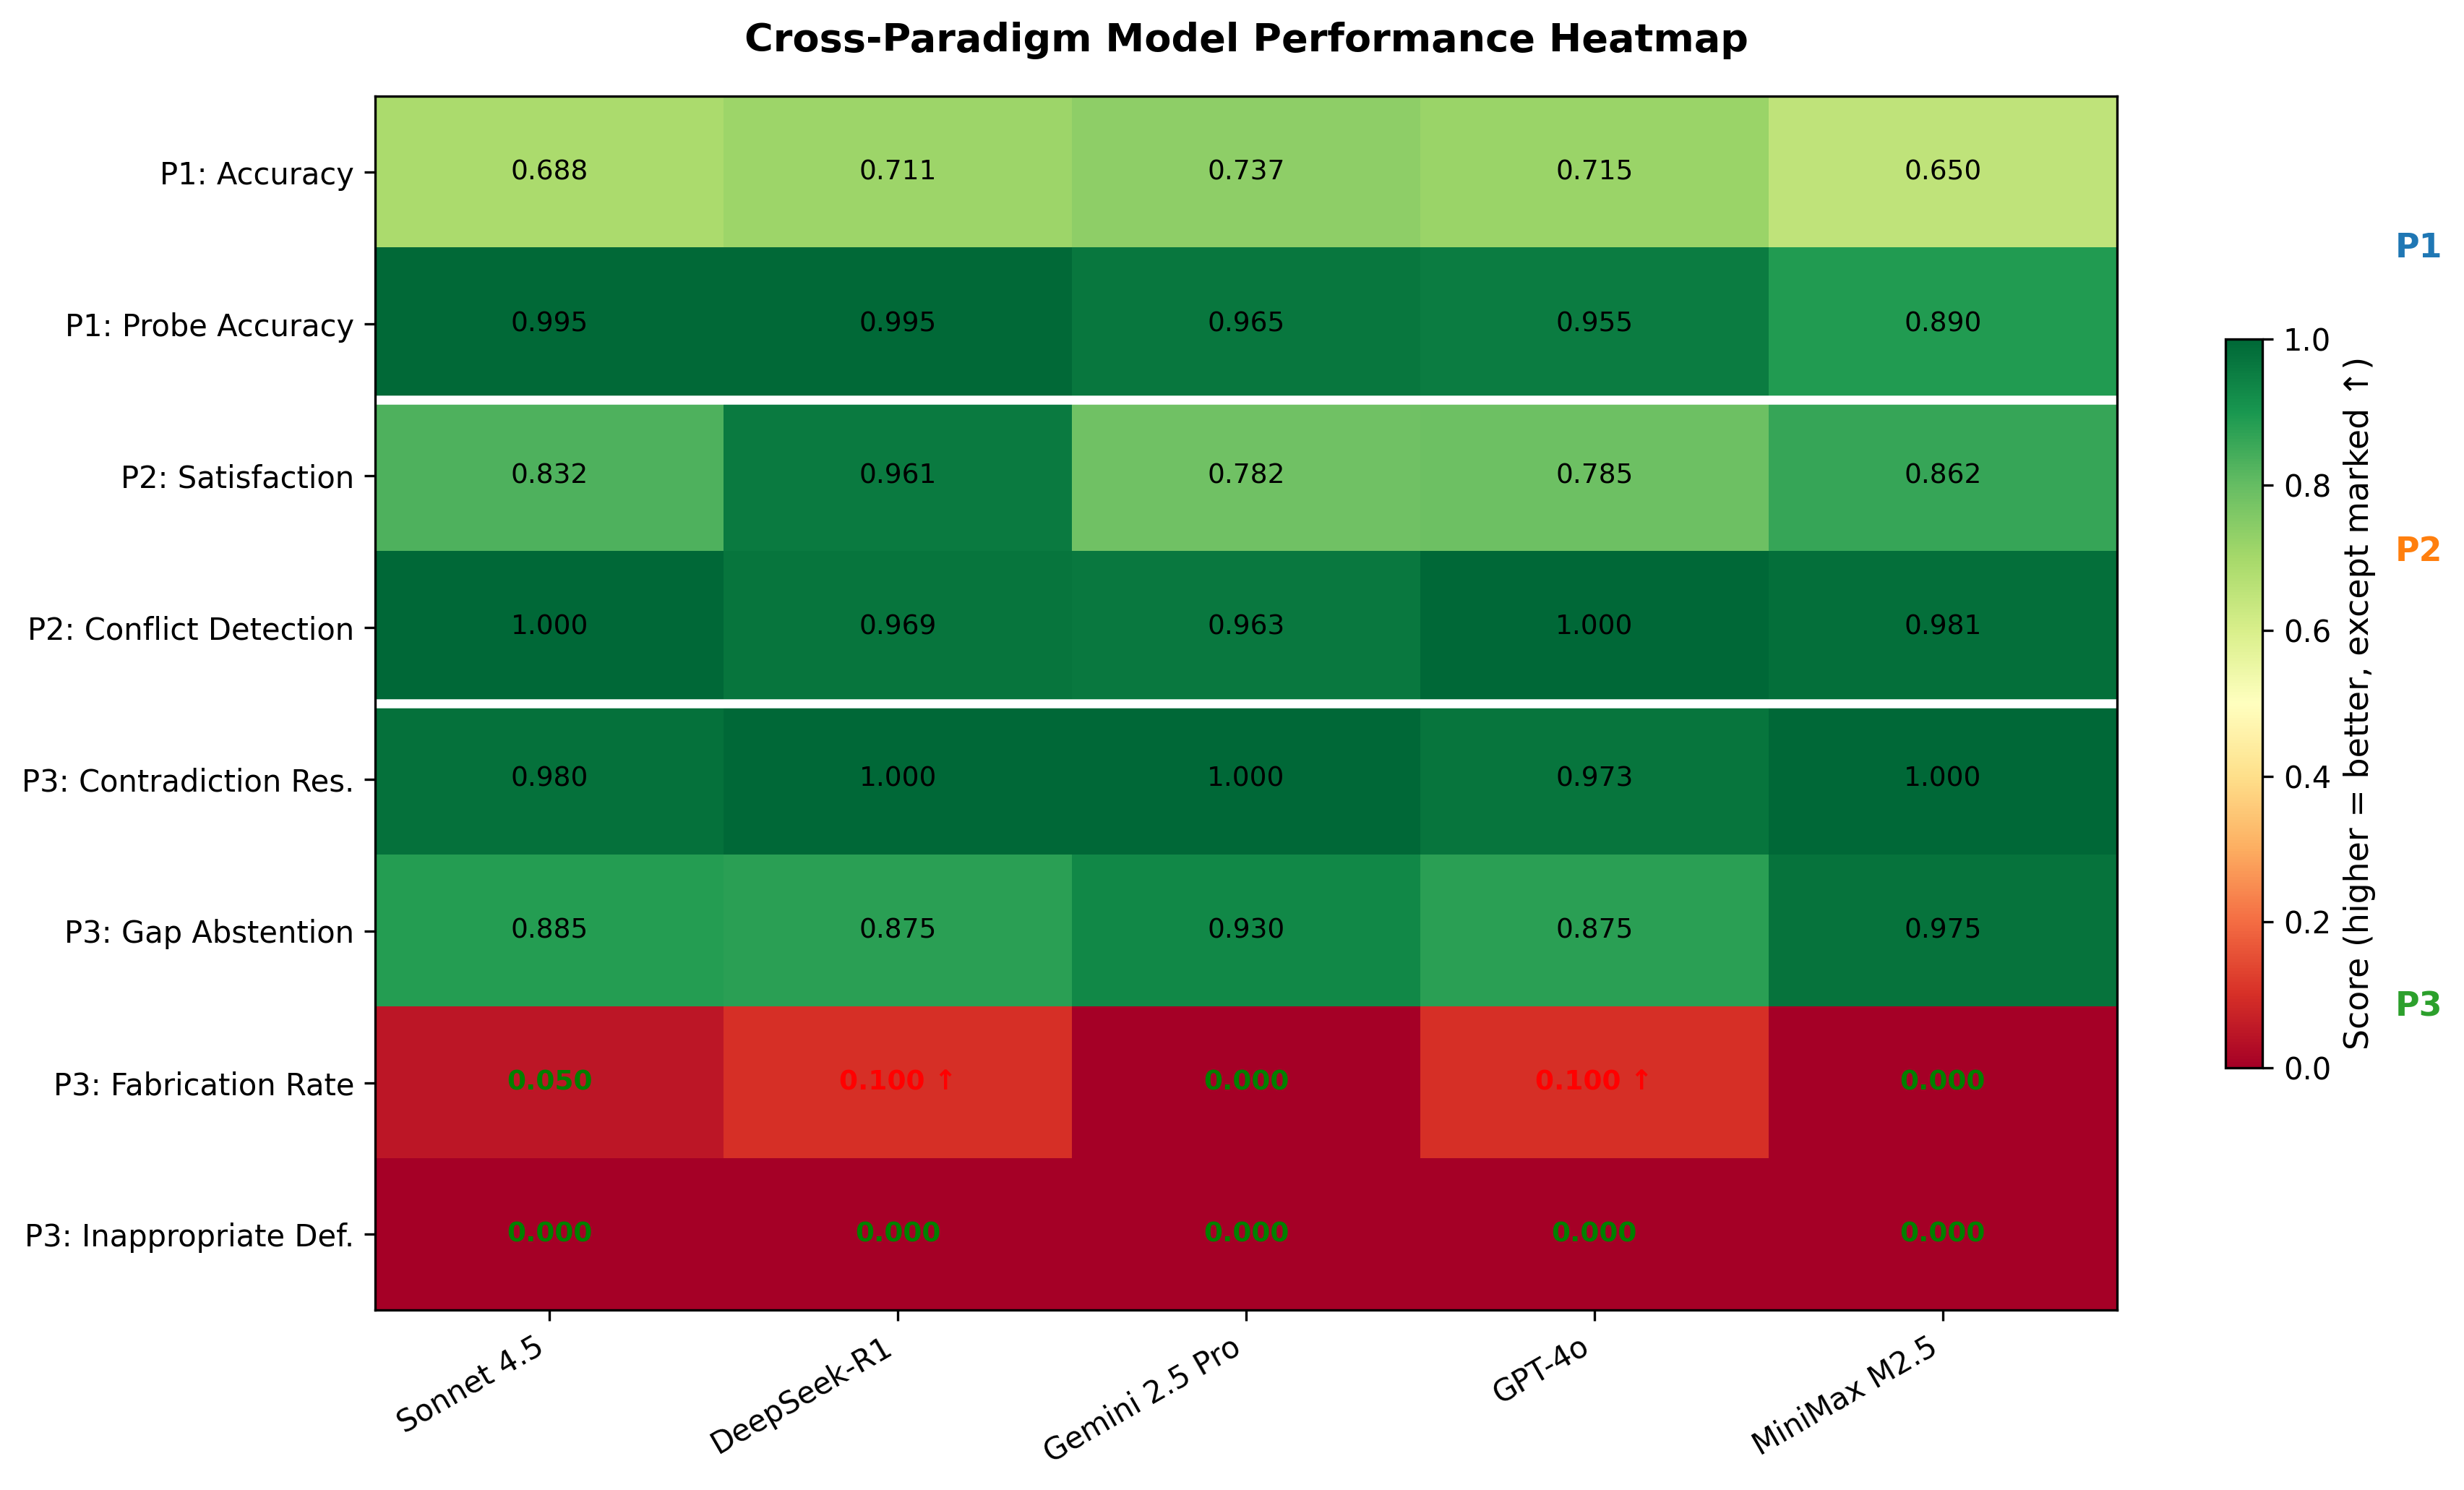
\includegraphics[width=\textwidth]{cross_paradigm_heatmap.png}
  \caption{Cross-paradigm heatmap. Green = higher; red = concerning. Rank inversions are pervasive.}
  \label{fig:heatmap}
\end{subfigure}
\hfill
\begin{subfigure}[t]{0.48\textwidth}
  \centering
  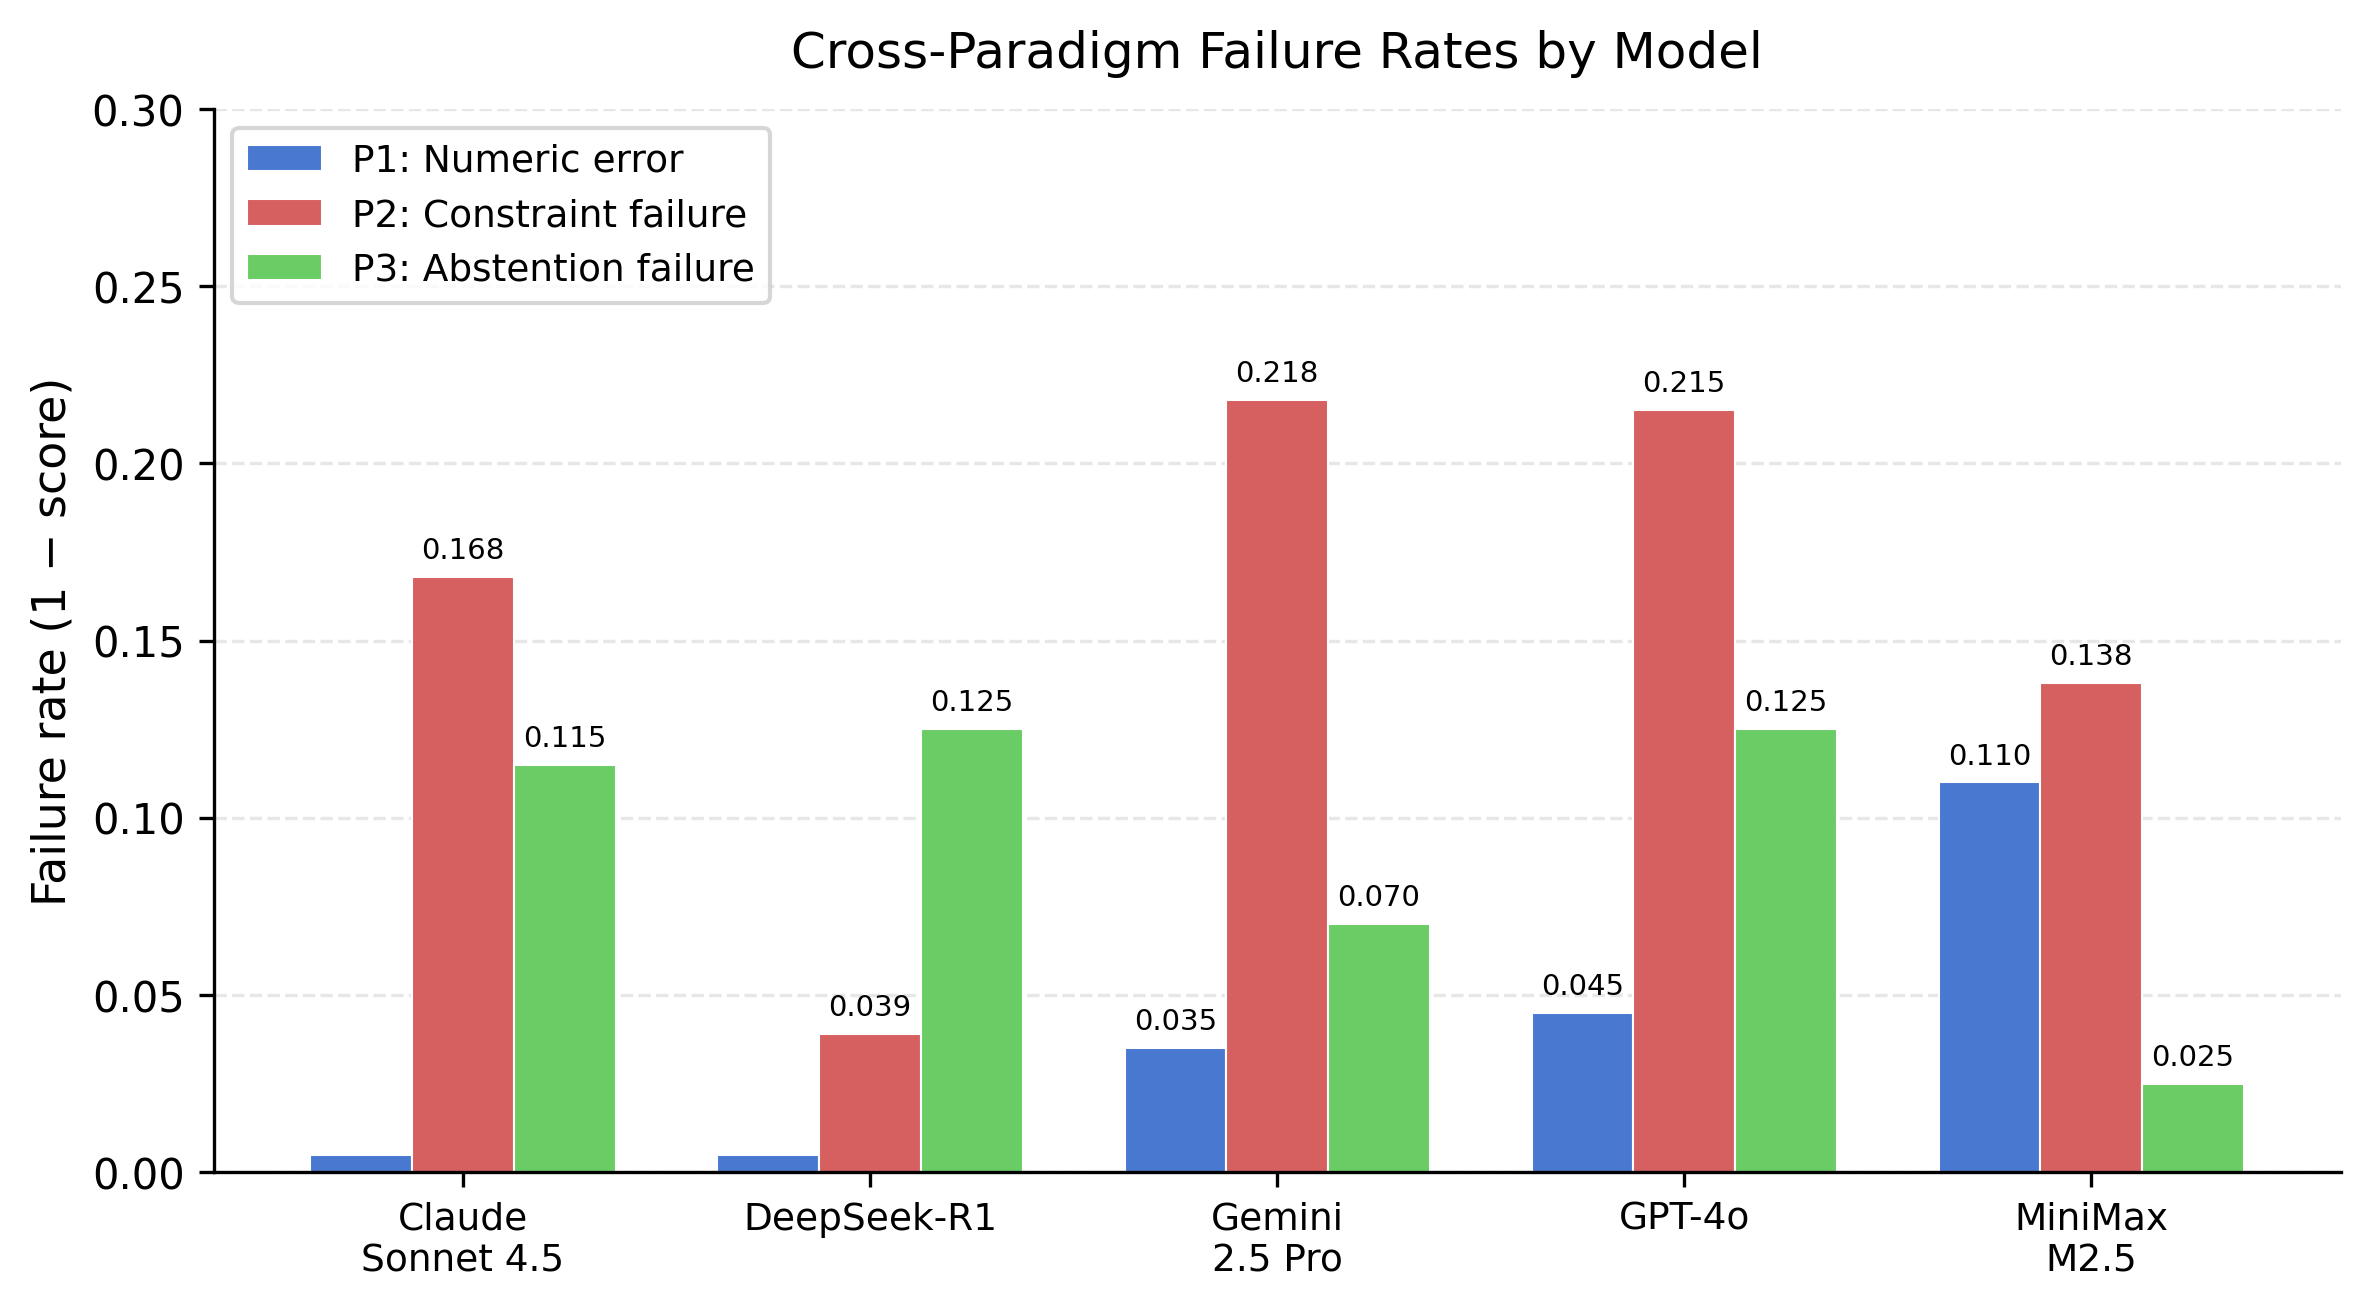
\includegraphics[width=\textwidth]{cross_paradigm_bar.png}
  \caption{Failure rates (1 $-$ score) by model and paradigm. Rank inversions are immediately visible: MiniMax~M2.5 has the highest P1 failure rate but the lowest P3 failure rate.}
  \label{fig:bar}
\end{subfigure}
\caption{Cross-paradigm performance visualizations. (a)~Heatmap of raw scores; (b)~failure rates highlighting the magnitude and direction of rank inversions across paradigms.}
\label{fig:cross-paradigm}
\end{figure*}

These concordance statistics are computed over $n = 5$ models, limiting statistical power. The P1--P3 inverse correlation survives conventional thresholds despite the small $n$, but should be confirmed with additional models. Crucially, the primary evidence for dissociability rests on within-paradigm decompositions: conflict detection versus integration in P2 (0.963--1.000 vs.\ 0.556--0.921 over hundreds of scored turns), and gap-type-specific fabrication in P3 (7.7\% for missing-evidence vs.\ 0--3.3\% for other types across 110 pairs). The cross-paradigm statistics provide a complementary summary, not the sole basis for the claim.

% ================================================================
\section{Discussion}
\label{sec:discussion}
% ================================================================

\paragraph{Hallucination as selective fragility.}
The central finding is that hallucination resistance comprises behaviorally dissociable competencies whose failures cannot be attributed to general context degradation. The P1 paradigm establishes that retrieval, revision integration, and recomputation remain intact across 20 turns. The significant inverse correlation between numeric fidelity and source fidelity ($\rho = -0.895$, $p = 0.040$) sharpens this, since these capabilities do not merely fail to covary but appear to trade off, with models best at precise numeric tracking being the most prone to epistemic overconfidence, though this pattern should be confirmed across a larger model sample.

\paragraph{Detection versus integration.}
The dissociation between understanding and applying, specifically uniformly high conflict detection (0.963--1.000) but widely varying integration (0.556--0.921), parallels findings in human cognition where detecting an inconsistency and resolving it are dissociable processes \citep{johnson1994sources}. The practical implication is that detection-based evaluations systematically overestimate model competence relative to integration-based evaluations.

\paragraph{Failure architecture is task-dependent.}
Models do not have fixed capability profiles. Gemini~2.5~Pro exhibits the strongest numeric computation (highest per-phase accuracy in P1) and the most brittle constraint architecture (steepest post-conflict collapse in P2). DeepSeek-R1 achieves the most consistent cross-paradigm performance (P1: 0.995, P2: 0.961, P3 contradiction resolution: 1.000). GPT-4o and Claude Sonnet~4.5 occupy middle ground with different trade-off profiles. These task-dependent profiles have practical implications. For instance, a model selected for financial analysis (where P1 demands dominate) may be poorly suited for project planning (where P2 demands dominate), even if both tasks superficially involve ``tracking information across conversation.''

\paragraph{Authority bias as conditionally solved.}
The zero inappropriate authority deference is reassuring but conditional. Our scenarios explicitly presented conflicting sources of different status, and whether models would resist subtler authority signals remains open. The mild over-skepticism in Claude Sonnet~4.5 and GPT-4o (14\% resistance to correct authority) may represent a calibration cost of robust deference resistance.

\paragraph{Implications for evaluation.}
Current leaderboards conflate empirically dissociable capabilities. A user selecting a model for financial analysis based on a composite trustworthiness score might choose one that excels at source fidelity but underperforms at constraint maintenance. Evaluation frameworks should separately report: (a)~multi-turn numeric fidelity, (b)~constraint maintenance under revision, and (c)~source fidelity with gap-type-specific fabrication rates. The behavioral dissociability we document means that aggregate scores obscure decision-relevant variation.

% ================================================================
\section{Conclusion}
\label{sec:conclusion}
% ================================================================

This paper demonstrates that hallucination resistance in frontier language models is not a single capability but comprises behaviorally dissociable failure modes with different task demands. Models that maintain near-perfect numeric fidelity across 20-turn conversations (0.890--0.995 probe accuracy) nonetheless fail dramatically at constraint integration after revision (dropping as low as 0.556 satisfaction) and fabricate selectively in response to specific gap structures (7.7\% for implied-evidence gaps across an expanded 13-scenario sample vs.\ 0--3.3\% for other types). These failures cannot be explained by general context degradation: P1 establishes that models can retrieve their own prior outputs, integrate revisions, and recompute derived values across the full conversation. The strongest cross-paradigm signal is a significant inverse correlation between numeric fidelity and source fidelity ($\rho = -0.895$, $p = 0.040$), suggesting these capabilities may trade off rather than merely vary independently.

Several limitations warrant acknowledgment. The cross-paradigm concordance statistics are computed over five models, limiting statistical power; the primary support for dissociability comes from within-paradigm decompositions computed over hundreds of data points, and from the significant P1--P3 inverse correlation that survives despite the small sample. P3 evaluation used an LLM judge (Claude Opus) from the same model family as one subject (Claude Sonnet~4.5). However, independent re-judgment of all 100 entries by GPT-5.2 (a model from a different provider) yielded 97.2\% agreement (AC1 $= 0.971$), providing cross-provider validation that the rubric produces consistent scores regardless of the judge model's provenance. Each model-scenario combination was run once, and specific rankings may shift with repeated runs or as providers update models. The gap-type analysis for non-evidence gap types rests on relatively small per-type samples ($N = 2$--6), but the missing-evidence sample was expanded from 5 to 13 scenarios as a pre-submission robustness check, and the gap-type specificity of fabrication held at the larger sample size, though the overall rate decreased from the initial estimate.

To assess sensitivity to the single-run design, we conducted a targeted replication of the 20 highest-variance and highest-stakes scenarios (100 conversations total, 5 models at temperature 0). The structural conclusions, name the behaviorally decomposable hallucination resistance and the divergent cross-paradigm rankings, were robust to re-evaluation. Specific satisfaction point estimates for closely-clustered models should be interpreted as approximate. Full replication details are in Appendix~\ref{app:replication}.

Our scenarios use planted contradictions, explicit gaps, and clearly attributed sources. In naturalistic settings, contradictions are implicit, gaps are unmarked, and authority signals are subtler. The direction of this bias is likely conservative, given implicit contradictions should be harder to detect than explicit ones, making our near-perfect detection rates an upper bound and the detection-integration gap a lower bound on the dissociation that would be observed in the wild. For fabrication, the direction is less certain. Naturalistic documents contain more unmarked implied-evidence structures, which could increase the frequency of implication-to-certainty collapse, but the absence of explicit gap framing might also reduce the triggering conditions. The structural finding, that hallucination resistance is multidimensional and behaviorally decomposable, is likely more durable than the specific effect sizes or model rankings.

\paragraph{Why might these capabilities dissociate?}
The three paradigms place structurally different demands on the model: in-context retrieval and arithmetic (P1), combinatorial search over a growing constraint space (P2), and reasoning about the \emph{absence} of evidence (P3). There is no a priori reason to expect a single training signal to optimize all three simultaneously. All five models were accessed via API, precluding inspection of architecture or training pipelines. Testing open-weight models would help distinguish whether the dissociation arises from architectural properties, RLHF objectives, or their interaction.

The practical implication is that there is no single trustworthy model, only models whose failure mode profiles match or mismatch specific tasks. We release our full experimental framework, scenario generators, and scored results to support replication and extension.

% ================================================================
% REFERENCES
% ================================================================

\begin{thebibliography}{20}

\bibitem[\protect\citeauthoryear{Artstein and Poesio}{2008}]{artstein2008inter}
Ron Artstein and Massimo Poesio.
\newblock 2008.
\newblock Inter-coder agreement for computational linguistics.
\newblock \emph{Computational Linguistics}, 34(4):555--596.

\bibitem[\protect\citeauthoryear{Chen et~al.}{2024}]{chen2024diahalu}
Kedi Chen, Qin Chen, Jie Zhou, He Yishen, and Liang He.
\newblock 2024.
\newblock {DiaHalu}: A dialogue-level hallucination evaluation benchmark for large language models.
\newblock In \emph{Findings of EMNLP}.

\bibitem[\protect\citeauthoryear{Chiang et~al.}{2024}]{chiang2024chatbot}
Wei-Lin Chiang, Lianmin Zheng, Ying Sheng, et~al.
\newblock 2024.
\newblock Chatbot {A}rena: An open platform for evaluating {LLM}s by human preference.
\newblock In \emph{Proceedings of ICML}.

\bibitem[\protect\citeauthoryear{Byrt et~al.}{1993}]{byrt1993bias}
Ted Byrt, Janet Bishop, and John~B. Carlin.
\newblock 1993.
\newblock Bias, prevalence and kappa.
\newblock \emph{Journal of Clinical Epidemiology}, 46(5):423--429.

\bibitem[\protect\citeauthoryear{Cohen}{1960}]{cohen1960coefficient}
Jacob Cohen.
\newblock 1960.
\newblock A coefficient of agreement for nominal scales.
\newblock \emph{Educational and Psychological Measurement}, 20(1):37--46.

\bibitem[\protect\citeauthoryear{Gwet}{2008}]{gwet2008computing}
Kilem~Li Gwet.
\newblock 2008.
\newblock Computing inter-rater reliability and its variance in the presence of high agreement.
\newblock \emph{British Journal of Mathematical and Statistical Psychology}, 61(1):29--48.

\bibitem[\protect\citeauthoryear{Ji et~al.}{2023}]{ji2023survey}
Ziwei Ji, Nayeon Lee, Rita Frieske, Tiezheng Yu, Dan Su, Yan Xu, Etsuko Ishii, Ye~Jin Bang, Andrea Madotto, and Pascale Fung.
\newblock 2023.
\newblock Survey of hallucination in natural language generation.
\newblock \emph{ACM Computing Surveys}, 55(12):1--38.

\bibitem[\protect\citeauthoryear{Johnson-Laird and Byrne}{1994}]{johnson1994sources}
P.~N. Johnson-Laird and Ruth M.~J. Byrne.
\newblock 1994.
\newblock Models, necessity, and the search for counterexamples.
\newblock \emph{Behavioral and Brain Sciences}, 17(4):775--778.

\bibitem[\protect\citeauthoryear{Kendall and Babington~Smith}{1939}]{kendall1939problem}
Maurice~G. Kendall and Bernard Babington~Smith.
\newblock 1939.
\newblock The problem of $m$ rankings.
\newblock \emph{The Annals of Mathematical Statistics}, 10(3):275--287.

\bibitem[\protect\citeauthoryear{Li et~al.}{2023}]{li2023halueval}
Junyi Li, Xiaoxue Cheng, Wayne~Xin Zhao, Jian-Yun Nie, and Ji-Rong Wen.
\newblock 2023.
\newblock {HaluEval}: A large-scale hallucination evaluation benchmark for large language models.
\newblock In \emph{Proceedings of EMNLP}.

\bibitem[\protect\citeauthoryear{Liang et~al.}{2023}]{liang2023helm}
Percy Liang, Rishi Bommasani, Tony Lee, et~al.
\newblock 2023.
\newblock Holistic evaluation of language models.
\newblock \emph{Transactions on Machine Learning Research}.

\bibitem[\protect\citeauthoryear{Lin et~al.}{2022}]{lin2022truthfulqa}
Stephanie Lin, Jacob Hilton, and Owain Evans.
\newblock 2022.
\newblock {TruthfulQA}: Measuring how models mimic human falsehoods.
\newblock In \emph{Proceedings of ACL}.

\bibitem[\protect\citeauthoryear{Liu et~al.}{2023}]{liu2023geval}
Yang Liu, Dan Iter, Yichong Xu, Shuohang Wang, Ruochen Xu, and Chenguang Zhu.
\newblock 2023.
\newblock {G-Eval}: {NLG} evaluation using {GPT-4} with better human alignment.
\newblock In \emph{Proceedings of EMNLP}.

\bibitem[\protect\citeauthoryear{Liu et~al.}{2024}]{liu2024lost}
Nelson~F. Liu, Kevin Lin, John Hewitt, Ashwin Paranjape, Michele Bevilacqua, Fabio Petroni, and Percy Liang.
\newblock 2024.
\newblock Lost in the middle: How language models use long contexts.
\newblock \emph{Transactions of the Association for Computational Linguistics}, 12:157--173.

\bibitem[\protect\citeauthoryear{Min et~al.}{2023}]{min2023factscore}
Sewon Min, Kalpesh Krishna, Xinxi Lyu, et~al.
\newblock 2023.
\newblock {FActScore}: Fine-grained atomic evaluation of factual precision in long form text generation.
\newblock In \emph{Proceedings of EMNLP}.

\bibitem[\protect\citeauthoryear{Rathore et~al.}{2026}]{rathore2026temporal}
Vidhi Rathore et~al.
\newblock 2026.
\newblock Temporal graph network: Hallucination detection in multi-turn conversation.
\newblock \emph{arXiv preprint arXiv:2601.03051}.

\bibitem[\protect\citeauthoryear{Srivastava et~al.}{2023}]{srivastava2023beyond}
Aarohi Srivastava, Abhinav Rastogi, Abhishek Rao, et~al.
\newblock 2023.
\newblock Beyond the imitation game: Quantifying and extrapolating the capabilities of language models.
\newblock \emph{Transactions on Machine Learning Research}.

\bibitem[\protect\citeauthoryear{Valmeekam et~al.}{2023}]{valmeekam2023planbench}
Karthik Valmeekam, Matthew Marquez, Alberto Olmo, Sarath Sreedharan, and Subbarao Kambhampati.
\newblock 2023.
\newblock {PlanBench}: An extensible benchmark for evaluating large language models on planning and reasoning about change.
\newblock In \emph{Proceedings of NeurIPS}.

\bibitem[\protect\citeauthoryear{Xie et~al.}{2024}]{xie2024travelplanner}
Jian Xie, Kai Zhang, Jiangjie Chen, Tinghui Zhu, Renze Lou, Yuandong Tian, Yanghua Xiao, and Yu Su.
\newblock 2024.
\newblock {TravelPlanner}: A benchmark for real-world planning with language agents.
\newblock In \emph{Proceedings of ICML}.

\bibitem[\protect\citeauthoryear{Zheng et~al.}{2023}]{zheng2023judging}
Lianmin Zheng, Wei-Lin Chiang, Ying Sheng, et~al.
\newblock 2023.
\newblock Judging {LLM}-as-a-judge with {MT-Bench} and {Chatbot Arena}.
\newblock In \emph{Proceedings of NeurIPS}.

\end{thebibliography}

% ================================================================
\appendix
\section{Inter-Rater Reliability}
\label{app:irr}

To validate the P3 LLM judge, all 100 entries (5 models $\times$ 20 scenarios) were independently re-judged by GPT-5.2 (OpenAI, \texttt{gpt-5.2}, reasoning effort: medium) using the identical rubric and scoring schema applied by the primary judge (Claude Opus~4.6). This cross-provider design tests whether the rubric produces consistent scores when applied by a frontier model from a different vendor, providing stronger validation than within-family replication.

Scores were binned into ordinal categories (low: $[0, 0.25)$, mid: $[0.25, 0.75)$, high: $[0.75, 1.0]$). Because three of five dimensions exhibit extreme marginal skew (nearly all entries scored ``high'' by both judges), Cohen's $\kappa$ is subject to the Feinstein--Cicchetti prevalence paradox \citep{byrt1993bias}, producing near-zero or negative values despite $\geq$95\% agreement. We therefore report Gwet's AC1 \citep{gwet2008computing} as the primary agreement statistic, which remains well-behaved under prevalence skew, alongside raw agreement and $\kappa$ where the latter is interpretable.

\begin{table}[tbp]
\centering
\caption{Inter-rater reliability: Claude Opus~4.6 vs.\ GPT-5.2 on all 100 P3 entries. AC1 is Gwet's prevalence-robust agreement coefficient. $\kappa_{\mathrm{lin}}$: Cohen's $\kappa$ with linear weighting (reported where marginal variance permits interpretation).}
\label{tab:kappa}
\small
\begin{tabular}{lcccc}
\toprule
\textbf{Dimension} & \textbf{Agree} & \textbf{AC1} & \textbf{$\kappa_{\mathrm{lin}}$} & \textbf{Note} \\
\midrule
Contr.\ identified & 100\% & 1.000 & undef.    & Prevalence \\
Contr.\ resolved   &  95\% & 0.949 & $-$0.013  & Prev.\ paradox \\
Reasoning quality  &  98\% & 0.980 & $-$0.010  & Prev.\ paradox \\
Gap abstention     &  96\% & 0.955 & 0.877     & Almost perfect \\
Fabrication        &  97\% & 0.967 & 0.712     & Substantial \\
\midrule
\textbf{Overall}   &  \textbf{97.2\%} & \textbf{0.971} & \textbf{0.718} & \\
\bottomrule
\end{tabular}
\end{table}

Table~\ref{tab:kappa} presents the full results. Overall binned agreement is 97.2\% across 400 paired dimension scores (4 continuous dimensions $\times$ 100 entries), with AC1 $= 0.971$. Gap abstention and fabrication, the two dimensions with sufficient marginal variance for standard $\kappa$, yield $\kappa_{\mathrm{lin}} = 0.877$ (almost perfect) and $\kappa = 0.712$ (substantial), respectively. Bootstrap 95\% confidence intervals (2{,}000 replicates) for gap abstention are AC1: $[0.907, 0.989]$, $\kappa_{\mathrm{lin}}$: $[0.735, 0.973]$.

The negative $\kappa$ values for contradiction resolution and reasoning quality reflect the prevalence paradox, not disagreement. Both judges assign nearly all entries to the ``high'' bin, leaving insufficient marginal variance for $\kappa$ to function. PABAK (prevalence-adjusted $\kappa$; \citealt{byrt1993bias}) for these dimensions is 0.925 and 0.970 respectively, consistent with the AC1 values.

Only three fabrication judgments (across two scenarios) disagreed: P3\_014 (GPT-4o), where Opus flagged fabrication and GPT-5.2 did not; and P3\_019 (Gemini~2.5~Pro, MiniMax~M2.5), where GPT-5.2 flagged fabrication and Opus did not. No systematic directional bias was observed, in contrast to the earlier human annotation study where the LLM judge was consistently stricter. Agreement was uniform across models: per-model binned agreement ranged from 95\% to 100\% on every dimension, confirming that no model's outputs were systematically harder to evaluate.

% ================================================================
\section{Targeted Replication}
\label{app:replication}

To assess sensitivity to the single-run design, we replicated the 20 highest-variance and highest-stakes scenarios (100 conversations total, 5 models at temperature 0; observed variation arises from GPU floating-point non-determinism and API-side batching differences rather than temperature sampling).

P1 probe scores agreed on 90\% of comparisons, with Gemini~2.5~Pro ranking first and MiniMax~M2.5 last in both runs; middle-tier models clustered within $\pm 0.05$ and swapped positions, consistent with sampling noise. P2 conflict detection was 96\% stable (48/50 identical), and the detection-integration dissociation held, as DeepSeek-R1 ranked first and Gemini~2.5~Pro last on post-conflict satisfaction in both runs. Individual P2 satisfaction point estimates on the hardest scenarios varied by up to 60 percentage points across runs, driven by output format variation crossing parsing thresholds. This instability affected the middle of the distribution while leaving extreme-position rankings intact.

For P3, fabrication judgments agreed on 23 of 25 scenario-model pairs (92\%). All three original fabrication instances (GPT-4o on two scenarios, DeepSeek-R1 on one) replicated on the same scenario-model pairs, all 20 non-fabricating pairs remained clean, and two pairs shifted from fabrication to partial abstention.

\end{document}
